\newpage
\section{Evaluierung des Featurevektors}
Der Featurevektor, der in dieser Arbeit verwendet wird, enthält 261 Merkmale. Wie diese ermittelt werden, wurde in Kapitel \ref{Aufbau} beschrieben. Jedes dieser Features soll dazu beitragen, die richtige Klasse für ein Sudoku zu finden.\\

\begin{figure}[H]
    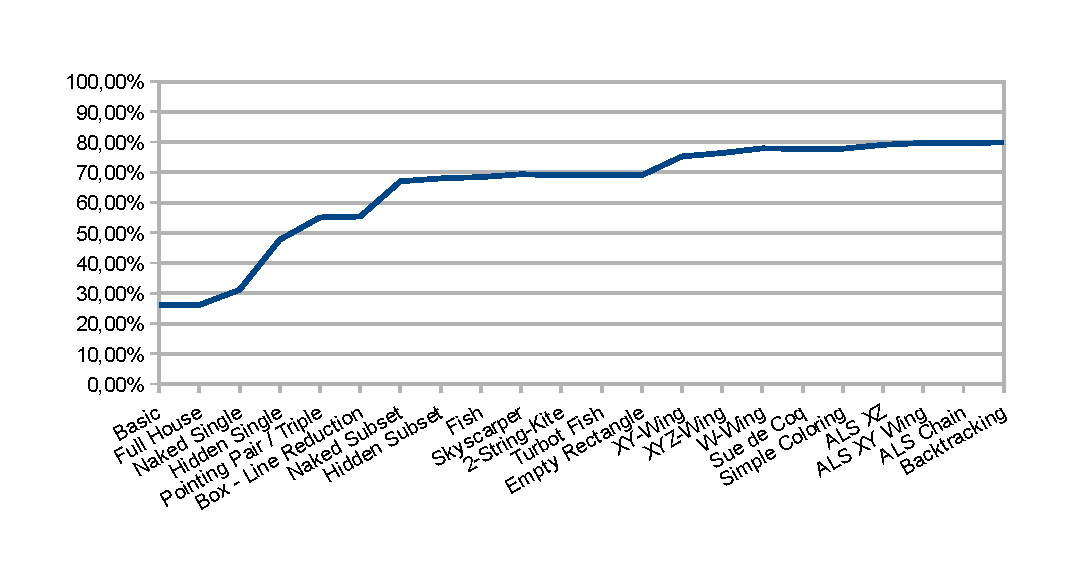
\includegraphics[width=\textwidth,height=\textheight,keepaspectratio]{./img/accuracy.eps}
    \caption{Genauigkeit des Klassifizierers bei Hinzunahme von Lösungsmethoden}
\end{figure}
\noindent In \textbf{Abbildung 5.2} steht \textit{Basic} für die Features, die ohne das Lösen des Sudokus extrahierbar sind, also zum Beispiel die Anzahl der vorgegebenen Ziffern. In der obigen Abbildung ist auf der X-Achse abgebildet, welche Features in den Featurevektor aufgenommen werden. Alle bis dahin aufgenommenen Features bleiben im Featurevektor, die neuen Features werden angehängt.\\
Zur Auswertung wurden 5000 Sudokus aus fünf unterschiedlichen Klassen verwendet. Das bedeutet, bei einer Einteilung in die Klassen mit Hilfe eines Zufallsgenerator läge die Genauigkeit im Schnitt bei 20\%.\\
Wenn man im Featurevektor nur die Merkmale hat, auf die ohne das Lösen des Sudokus gefunden werden können, dann liegt die Genauigkeit bereits bei über 26\%. Durch die Hinzunahme der Lösungsmethoden, die im Sudoku Ziffern ausfüllen, wird eine Genauigkeit von 47,7\% erzielt. Um dieses Ergebniss genauer interpretieren zu können, ist ein Blick auf die Konfusionsmatrizen des Klassifikators notwendig.\\

\begin{figure}[H]
\centering
\begin{tabular}{ l | l |  c  c  c  c  c | l}
\multicolumn{7}{c}{\textbf{Zugeordnete Klasse}}\\
\cline{2-7}
\multirow{6}{*}{\begin{turn}{90}\textbf{Ursprüngliche Klasse}\end{turn}}
 &  & a & b & c & d & e\\
\cline{2-7}
& a & 1000 & 0 & 0 & 0 & 0 & a = Easy \\
& b & 0 & 568 & 115 & 93 & 224 & b = Middle \\
& c & 0 & 288 & 333 & 221 & 158 & c = Hard \\
& d & 0 & 309 & 257 & 225 & 209 & d = Unfair \\
& e & 0 & 415 & 149 & 177 & 259 & e = Extreme \\
\cline{2-7}
\end{tabular}
\caption{Konfustionsmatrix mit einschließlich \textit{Hidden Single} Methode}
\end{figure}

\newpage
\noindent Wie man an \textbf{Abbildung 5.3} ablesen kann, ist der Klassifikator für Klasse a fehlerfrei und für b deutlich besser als für c, d und e. Der Klassifikator funktioniert also für einfache Sudokus besser als für schwere. Das ist so, weil in der momentanen Konfiguration nicht alle Features im Featurevektor sind, sondern nur die, die durch einfache Lösungsmethoden errechnet werden können. 

\begin{figure}[H]
    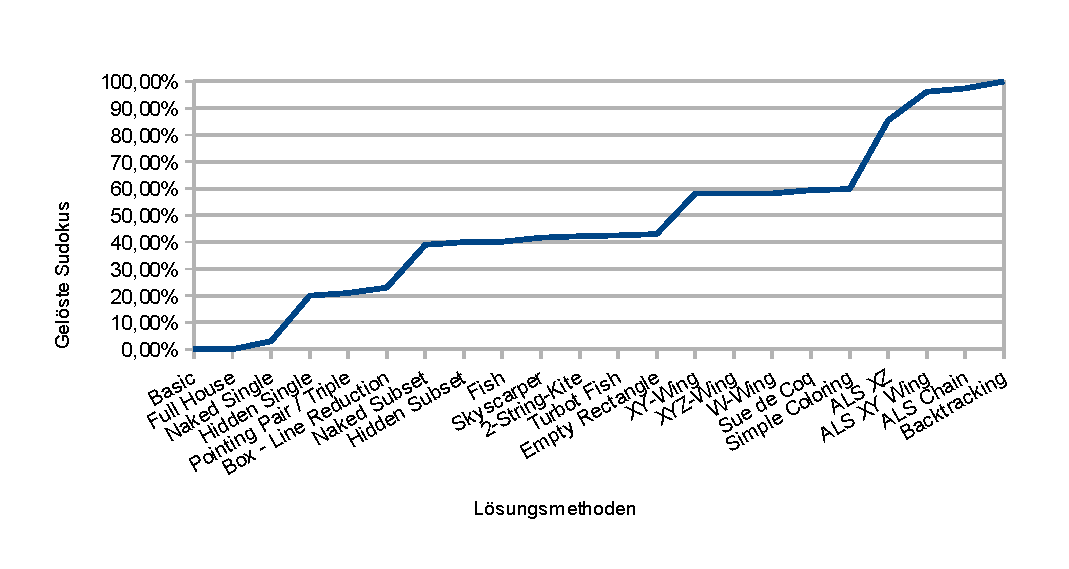
\includegraphics[width=\textwidth,height=\textheight,keepaspectratio]{./img/solvedcount.eps}
    \caption{Anzahl der gelösten Sudokus bei Hinzunahme von Lösungsmethoden}
\end{figure}

\noindent Aus \textbf{Abbildung 5.4} kann man entnehmen, dass die Anteil der gelösten Sudokus steigt, je mehr Lösungsmethoden angewendet werden. Da momentan nur Lösungsmethoden bis zur Technik \textit{Hidden Single} (\ref{Hidden Single}) angewendet werden, können nur leichte Sudokus (20\% der Gesamtmenge) gelöst werden und damit ist nur deren Featurevektor vollständig. Daher funktioniert die Unterschiedung nur zwischen leichten und schwereren Sudokus, eine genaue Unterscheidung innerhalb der schwereren Sudokus ist dem Klassifikator derzeit nicht möglich, da die Featurevektoren zu ähnlich sind. Mit der Hinzunahme von schwereren Lösungsmethoden lässt sich dieses Problem beheben.\\
Wenn man die Features in den Featurevektor aufnimmt, die von etwas schwereren Methoden generiert werden, dann sieht man wieder eine Steigerung der Genauigkeit in \textbf{Abbildung 5.3}. Nimmt man die Methoden bis einschließlich \textit{Hidden Subset} (\ref{Hidden Subset}) dazu, dann liegt der prozentuale Anteil der richtig klassifizierten Sudokus bei 67,98\%. Es können nun auch deutlich mehr Sudokus gelöst werden, genau 2005 Stück, was 40,1\% der gesamten Testmenge entspricht.\\
Hierdurch bedingt wird auch die Unterscheidung zwischen Sudokus in schwereren Klassen deutlicher. Da 40\% der Sudokus gelöst werden können, ist auch ihr Featurevektor vollständig. Wenn ein Sudoku mit den angewendeten Lösungsmethoden nicht gelöst werden kann, dann wird der bis dorthin erzeugt Featurevektor dem Klassifikator übergeben. Da es sich aber hier nur um Informationen handelt, die leichte Lösungsmethoden betreffen, ähneln sich die Featurevektoren der unlösbaren Sudokus stark.\\
\newpage
\begin{figure}[H]
\centering
\begin{tabular}{ l | l |  c  c  c  c  c | l}
\multicolumn{7}{c}{\textbf{Zugeordnete Klasse}}\\
\cline{2-7}
\multirow{6}{*}{\begin{turn}{90}\textbf{Ursprüngliche Klasse}\end{turn}}
 &  & a & b & c & d & e\\
\cline{2-7}
& a & 1000 & 0 & 0 & 0 & 0 & a = Easy \\
& b & 0 & 1000 & 0 & 0 & 0 & b = Middle \\
& c & 1 & 4 & 518 & 249 & 228 & c = Hard \\
& d & 1 & 0 & 312 & 299 & 388 & d = Unfair \\
& e & 0 & 0 & 174 & 244 & 582 & e = Extreme \\
\cline{2-7}
\end{tabular}
\caption{Konfustionsmatrix mit einschließlich \textit{Hidden Subset} Methode}
\end{figure}

\noindent In \textbf{Abbildung 5.5} sieht man die Konfusionsmatrix, die vom Klassifikator erzeugt wird, wenn man Lösungsmethoden bis einschließlich \textit{Hidden Subset} (\ref{Hidden Subset}) zum Lösen der Sudokus verwendet.\\
Hier sieht man eine deutliche Verbesserung in der Klasse b. Alle Sudokus, die aus Klasse b kommen, werden auch richtig als solche erkannt.\\
Mit den bisher verwendeten Lösungsmethoden können Sudokus aus den Klassen a und b komplett gelöst werden, aus Klasse c werden von 1000 Sudokus nur fünf gelöst und in den Klassen d und e kein Einziges. Im Vergleich zu \textbf{Abbildung 5.3} ist eine Verbesserung in Klasse c sichtbar, über die Hälfte der Sudokus aus Klasse c wurden korrekt klassifiziert, wobei es davor nur ein drittel waren. Das liegt vor allem daran, dass Sudokus aus Klasse c nicht mehr fälschlicherweise Klasse b zugeordnet werden. Die Sudokus aus Klasse d sind sehr stark in andere Klassen gestreut, jedoch werden die Sudokus fast ausschließlich in benachbarte Klassen eingeordnet.\\
Man kann hier deutlich erkennen, dass es eine starke Korrelation zwischen vollständig gelösten Sudokus und korrekt klassifizierten Sudokus gibt. Das liegt an der Vollständigkeit der Featurevektoren für die ersten beiden Klassen. Die starke Streuung in Klasse d resultiert daraus, dass es für diese Klasse keine klare Abgrenzung in eine Richtung gibt, was bei den Klasse c und e anders ist.\\
Der nächste große Sprung im Gewinn der Klassifikationsgenauigkeit ist nach dem Hinzunehmen der \textit{Wing-Techniken} (\ref{Wing}) zu erkennen. Hier steigt der Anteil der korrekt klassifizierten Sudokus auf knapp 78\%. Aus der Klasse c können nun 799 von 1000 Sudokus gelöst werden. Bei der Klasse d sind es fast 100 Sudokus und in Klasse e 13. Der Anteil der gelösten Sudokus steigt auf über 58\%, wie man auf \textbf{Abbildung 5.4} ablesen kann.\\
\begin{figure}[H]
\centering
\begin{tabular}{ l | l |  c  c  c  c  c | l}
\multicolumn{7}{c}{\textbf{Zugeordnete Klasse}}\\
\cline{2-7}
\multirow{6}{*}{\begin{turn}{90}\textbf{Ursprüngliche Klasse}\end{turn}}
 &  & a & b & c & d & e\\
\cline{2-7}
& a & 1000 & 0 & 0 & 0 & 0 & a = Easy \\
& b & 0 & 1000 & 0 & 0 & 0 & b = Middle \\
& c & 24 & 28 & 750 & 144 & 54 & c = Hard \\
& d & 4 & 1 & 104 & 507 & 384 & d = Unfair \\
& e & 0 & 0 & 17 & 344 & 639 & e = Extreme \\
\cline{2-7}
\end{tabular}
\caption{Konfustionsmatrix mit einschließlich \textit{W-Wing} Methode}
\end{figure}
\noindent In der Zugehörigen Konfusionsmatrix in \textbf{Abbildung 5.6} sieht man einen Anstieg der Klassifikationsgenauigkeit vor allem in den Klassen c und d, einen leichten Anstieg gibt es auch in Klasse e. Dies begründet sich damit, dass Sudokus der Klasse c nun in den meißten Fällen gelöst werden können. Dadurch ist ihr Featurevektor meißtens vollständig und damit besser von den Featurevektoren der anderen Klassen zu unterscheiden. Der Anstieg in der Klasse d kommt zustande, da Sudokus aus der Klasse d nun kaum noch fälschlicherweise in die Klasse c kategorisiert werden, da sich durch das Lösen von Sudokus aus Klasse c die Featurevektoren mehr voneinander unterscheiden.
Wenn man nun alle in dieser Arbeit verwendeten Lösungsmethoden in dem, in Kapitel \ref{Aufbau} beschriebenen, Algorithmus verwendet, dann werden 100\% der Sudokus gelöst. Allerdings müssen 2,6\% davon mit \textit{Backtracking} gelöst werden. \textit{Backtracking} ist ein Sonderfall der Lösungsmethoden. Es trägt nicht eine Ziffer ein oder löscht einige Kandidaten aus den Kandidatenlisten der Felder wie andere Lösungsmethoden, \textit{Backtracking} löst das ganze Sudoku auf einmal. Daher lassen sich daraus nicht viele Informationen über den Schwierigkeitsgrad des Sudokus ziehen. Da \textit{Backtracking} erst verwendet wird, wenn keine andere Lösungsmethode mehr funktioniert, kann man sagen, dass das Sudoku für die meißten menschlichen Spieler unlösbar wäre. Dazu ist zu sagen, dass es noch andere Lösungsmethoden gibt, die auch einige schwerere Sudokus lösen können und dass Backtracking auch unter sehr großem Zeitaufwand von menschlichen Spielern durchgeführt werden kann. Betrachtet man den Informationsgewinn nach dem Hinzufügen der \textit{W-Wing} Methode bis zum \textit{Backtracking}, dann sieht man einen Genauigkeitsgewinn von unter 2\%. Um diesen Gewinn zu erzielen, mussten 54 Features in den Featurevektor aufgenommen werden. Der Gewinn ist also sehr niedrig im Vergleich zum Aufwand, obwohl zusätzliche 38\% der Sudokus gelöst werden können, wobei hier \textit{Backtracking} nicht betrachtet wurde.\\

\begin{figure}[H]
\centering
\begin{tabular}{ l | l |  c  c  c  c  c | l}
\multicolumn{7}{c}{\textbf{Zugeordnete Klasse}}\\
\cline{2-7}
\multirow{6}{*}{\begin{turn}{90}\textbf{Ursprüngliche Klasse}\end{turn}}
 &  & a & b & c & d & e\\
\cline{2-7}
& a & 1000 & 0 & 0 & 0 & 0 & a = Easy \\
& b & 0 & 999 & 1 & 0 & 0 & b = Middle \\
& c & 1 & 35 & 785 & 145 & 34 & c = Hard \\
& d & 0 & 10 & 129 & 636 & 225 & d = Unfair \\
& e & 0 & 0 & 14 & 367 & 619 & e = Extreme \\
\cline{2-7}
\end{tabular}
\caption{Konfustionsmatrix mit allen vorgestellten Lösungsmethoden}
\end{figure}

\noindent Die Konfusionsmatrix, die erzeugt wird, wenn alle vorgestellten Methoden angewendet werden, ist in \textbf{Abbildung 5.7} zu sehen. Hier sieht man eine Verbesserung in den Klassen c, d und e. 116 Sudokus der Klasse e können mit den verwendeten Lösungsmethoden ohne \textit{Backtracking} nicht gelöst werden. Die schlechteren Ergebnisse in dieser Klasse gegenüber den Klassen mit leichterem Schwierigkeitsgrad, sind mit der Unvollständigkeit des Featurevektors zu begründen.
